%================================================================
\section{Introduction}

% XXX - maybe update this intro for ICIDS.
The computational generation of stories (hereafter {\em narrative
generation}) can help us understand some of the most creative aspects of
human intelligence~\cite{boyd2009origin}, such as reasoning about possible
and impossible worlds, and weaving narratives around our daily
lives~\cite{herman2013storytelling}.  Historically, narrative generation
has followed what Ronfard and Szilas \cite{ronfard2014story} term the
\emph{pipeline model}: a narrative artifact is generated by
first simulating the story world to form a collection of events, and then piping
the event information to a discourse generator, which generates a
selective presentation of story world events in a particular medium. A great
deal of existing work in narrative generation has primarily pursued this
pipeline model~\cite{gervas2009computational}. 
% XXX - update citation for ICIDS?

However, as Ronfard and Szilas argue, the pipeline model is neither
necessary nor sufficient for narrative generation.  Human authors
intentionally design their narratives to affect audiences in specific ways,
which involves reasoning about how story events are communicated more than
which story events occur~\cite{chatman1980story,bordwell1989making}. It is
unnecessary to simulate an aspect of the narrative universe that is never
communicated to the audience, if it does not inform the ultimate delivery
of the narrative artifact. It is also insufficient to reason about story
independent from discourse and medium, as the characteristics of a
discourse realization constrain the stories that can be told in that
medium~\cite{herman2004toward}.  The pipeline model unnecessarily restricts
how creative the generator can ultimately be, since story world commitments
are not revisited when generating discourse. Further, as will be detailed
later, narrative authorship depends on audiences being able to fill in the
gaps left open in the consumption of a
story~\cite{saraceni2016relatedness,magliano2016filling}.

Most prior work that uses the pipeline model implicitly assumes text, or
spoken verbal language, as the output generation medium, which allows the
pipeline model to avoid some of its limitations by baking medium
assumptions into the story model. For example, narrative generators can
model updates to internal character state, such as emotion or knowledge
change, which can simply be described in text. Communicating those
occurrences visually poses a significantly greater challenge.
Thus, we propose a simple kind of {\em visual} narrative as a testbed for
discourse generation: wordless comics, as in Figure~\ref{fig:calvin}. 
Comics are a relatively unexplored
domain of computational narratology~\cite{mani2012computational}, and they
present a wide range of expressive opportunities not afforded by text.

\begin{figure}
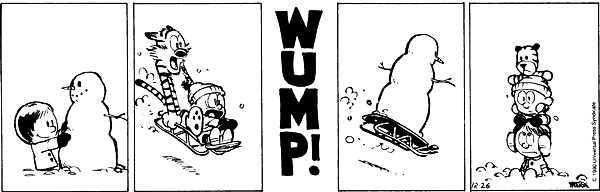
\includegraphics[width=\columnwidth]{calvin-and-hobbes.png}
\caption{
This wordless Calvin and Hobbes comic strip (\copyright Bill Watterson)
exemplifies the domain we are targeting with our generator. The strip also
illustrates how little plot structure informs this kind of short-form visual
storytelling.
}
\label{fig:calvin}
\end{figure}

Our work represents a departure from the pipeline model, a
\emph{discourse-driven} approach to narrative generation, for generating
comics. In this model, the story world is only simulated inasmuch as is
necessary to support the telling of story events in the discourse; that is,
we have a notion of temporal ordering and account for which actants have
previously appeared. We present a small-scale computational
system~\cite{montfort2012small} to generate comics as a proof-of-concept
for our approach.

In the remainder of this paper, we discuss theoretical aspects of comics
authoring, our computational implementation of a comic generation system,
and our experience with refining our model with linguistic constraints. Our
primary takeaway is that both global and local reasoning are important
aspects of narrative generation: local reasoning is important for
maintaining narrative coherence, and global reasoning is important for
maintaining satisfying narrative structure. Both are thus important parts
of creating comprehensible comics, and we present an outline of future work
designed to explore the human interpretation of our generated artifacts.

